\section{Results}\label{sec:results}
In this section, we describe the results of our experiment. 

\begin{figure}[t!]
\centering
\subfigure[North America.]{%
\label{fig:Ohio_NA}%
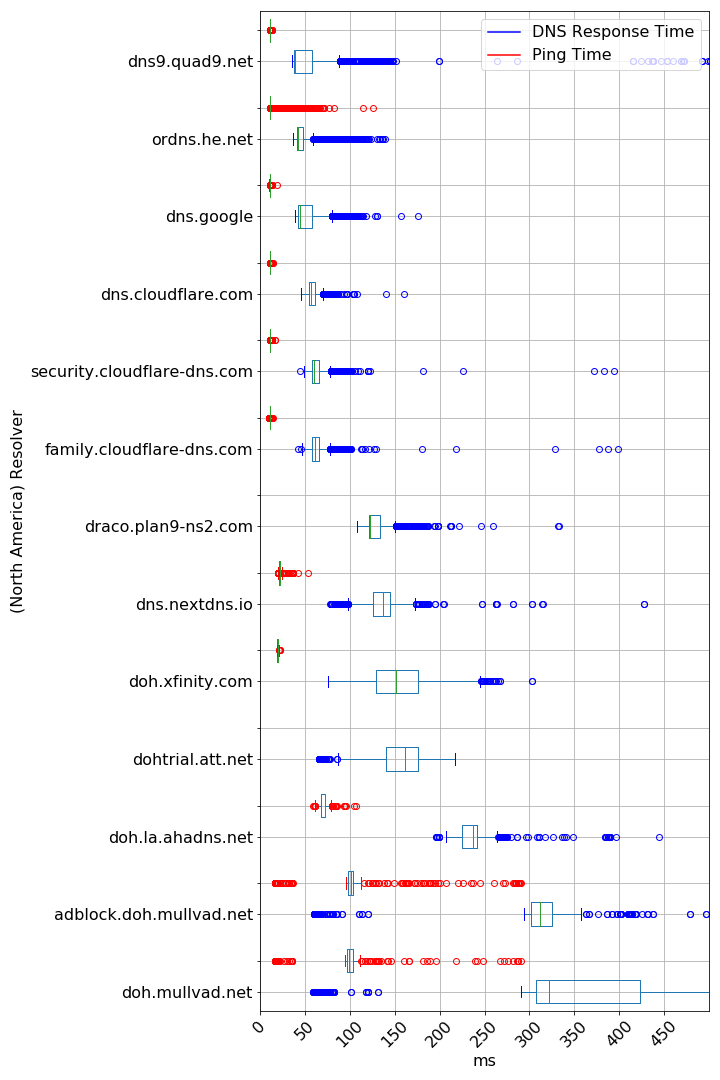
\includegraphics[height=2in]{figures/Ohio_North_America.png}}%
\hspace{8pt}%
\subfigure[Asia.]{%
\label{fig:Ohio_Asia}%
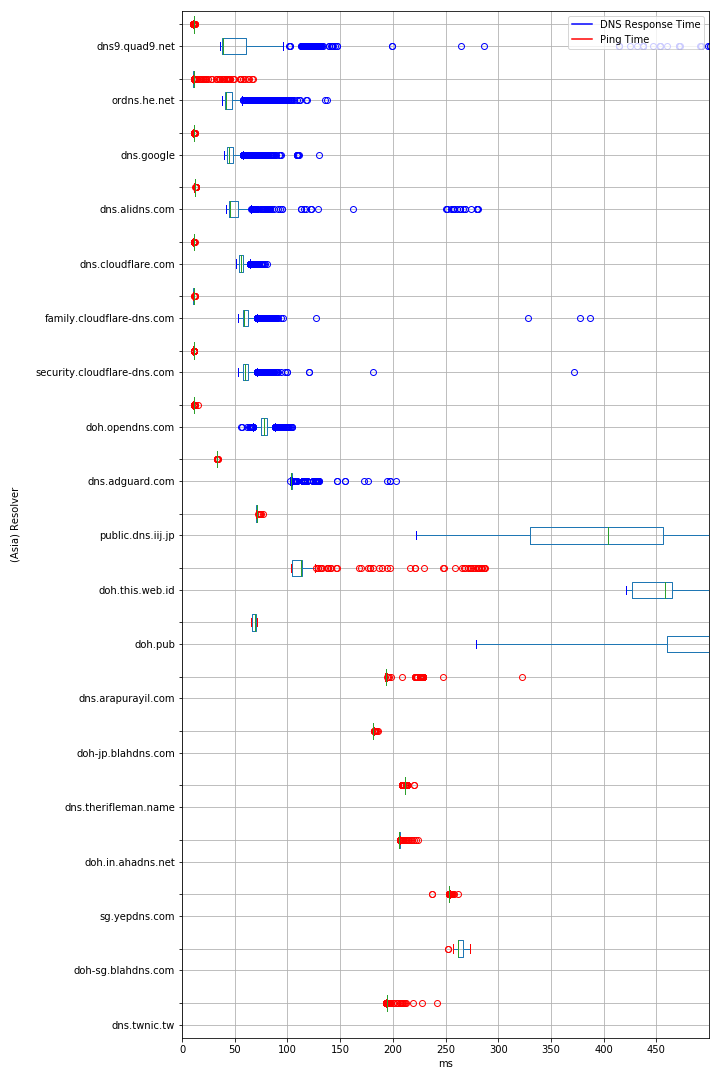
\includegraphics[height=2in]{figures/Ohio_Asia.png}}%
\hspace{8pt}%
\subfigure[Europe.]{%
\label{fig:Ohio_Europe}%
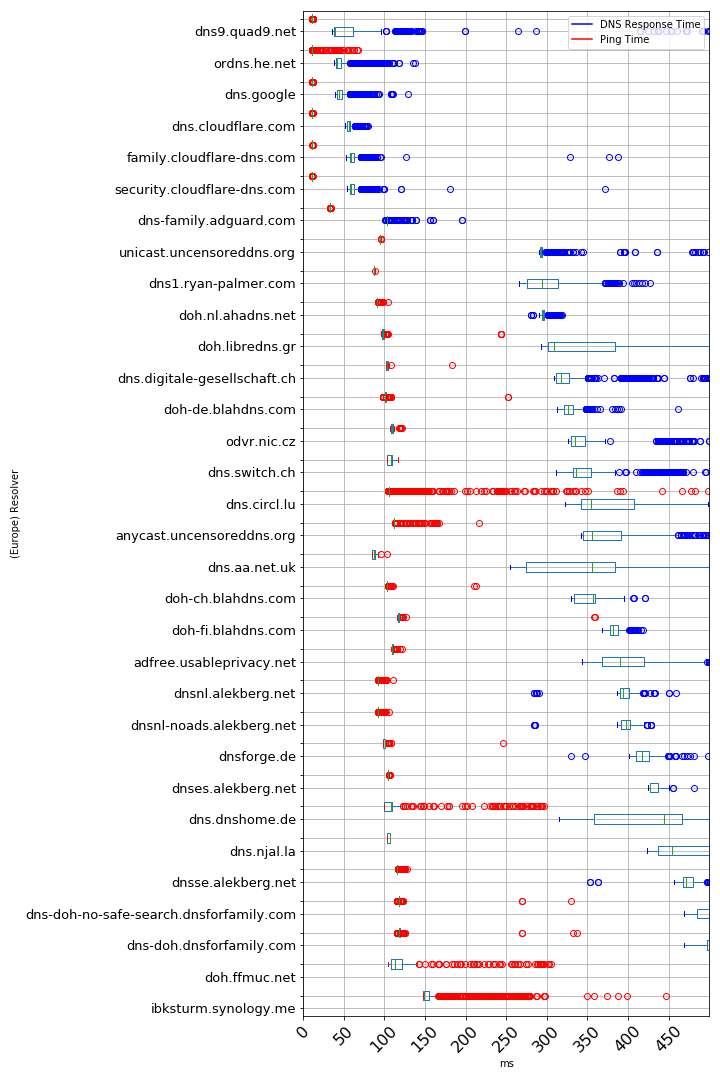
\includegraphics[height=2in]{figures/Ohio_Europe.png}}%
\caption{Resolvers measured from a vantage point in Ohio, USA.}
\end{figure}

\begin{figure}[t!]
\centering
\subfigure[North America.]{%
\label{fig:Seoul_NA}%
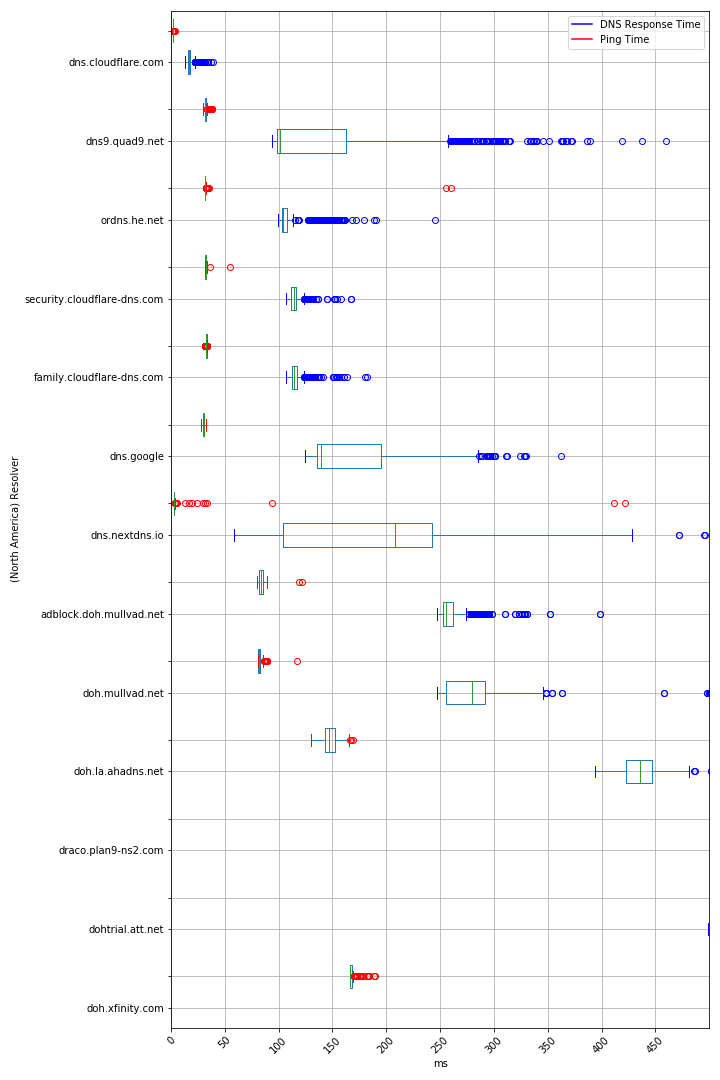
\includegraphics[height=2in]{figures/Seoul_North_America.png}}%
\hspace{8pt}%
\subfigure[Asia.]{%
\label{fig:Seoul_Asia}%
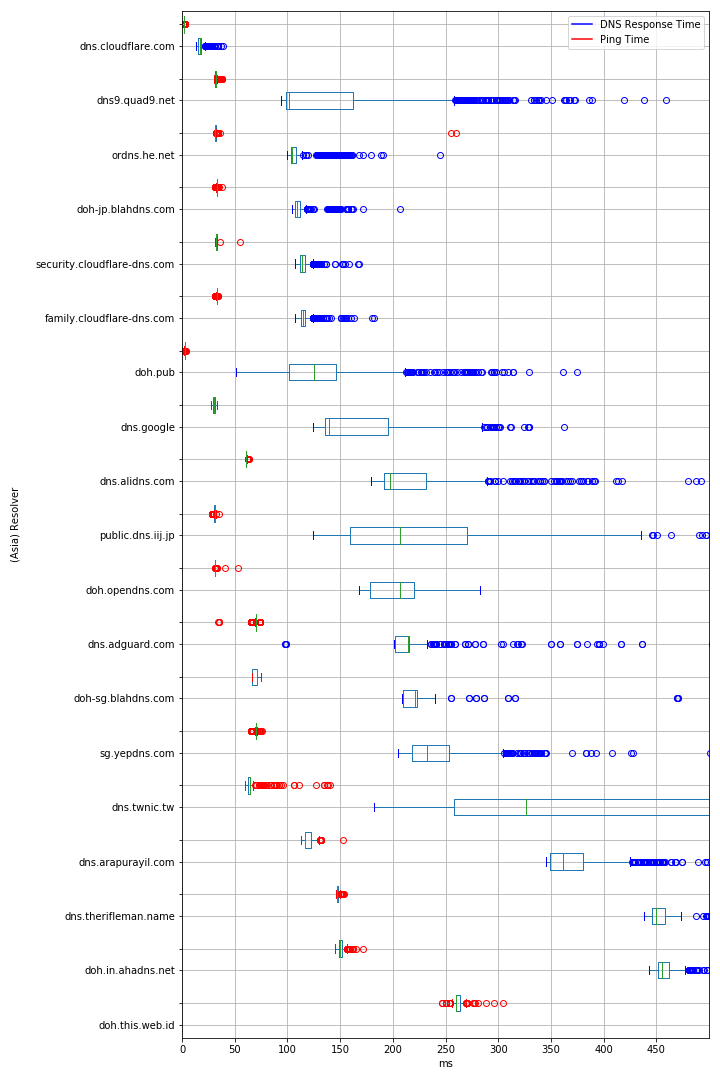
\includegraphics[height=2in]{figures/Seoul_Asia.png}}%
\hspace{8pt}%
\subfigure[Europe.]{%
\label{fig:Seoul_Europe}%
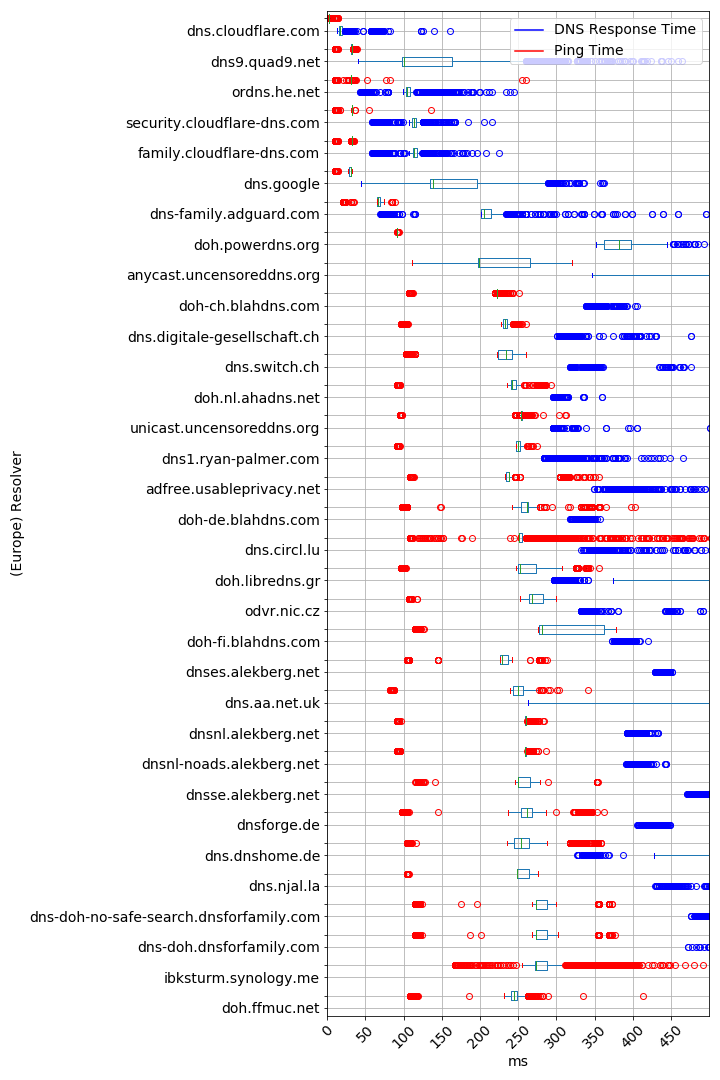
\includegraphics[height=2in]{figures/Seoul_Europe.png}}%
\caption{Resolvers measured from a vantage point in Seoul, South Korea.}
\end{figure}

\begin{figure}[t!]
\centering
\subfigure[North America.]{%
\label{fig:Frankfurt_NA}%
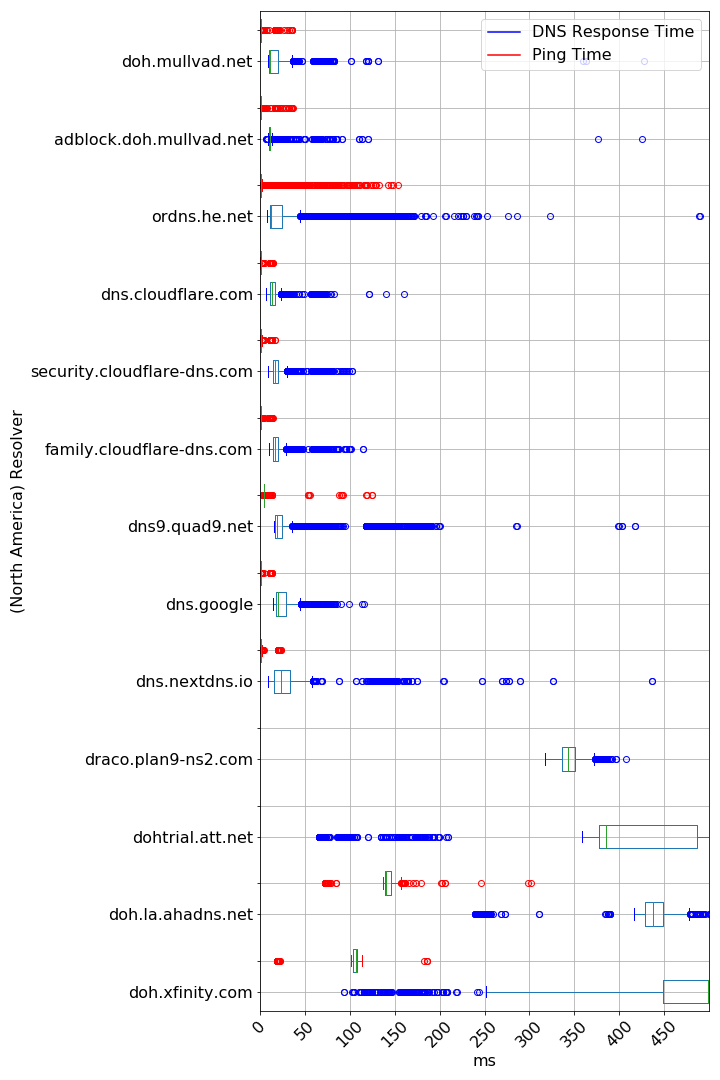
\includegraphics[height=2in]{figures/Frankfurt_North_America.png}}%
\hspace{8pt}%
\subfigure[Asia. ]{%
\label{fig:Frankfurt_Asia}%
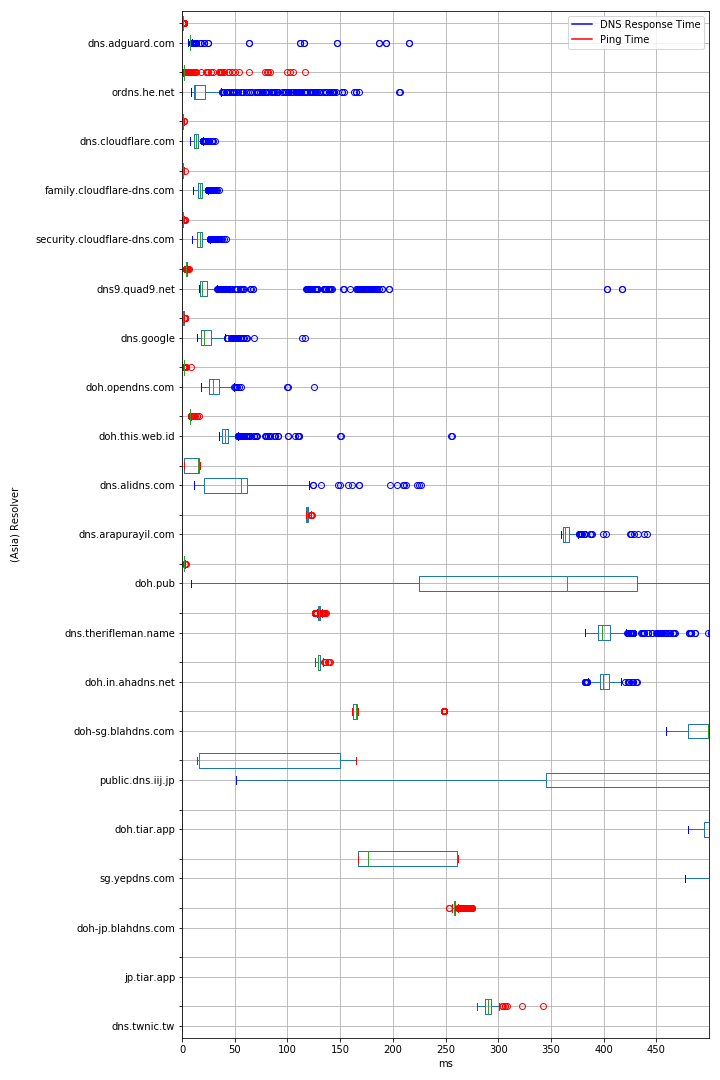
\includegraphics[height=2in]{figures/Frankfurt_Asia.png}}%
\hspace{8pt}%
\subfigure[Europe.]{%
\label{fig:Frankfurt_Europe}%
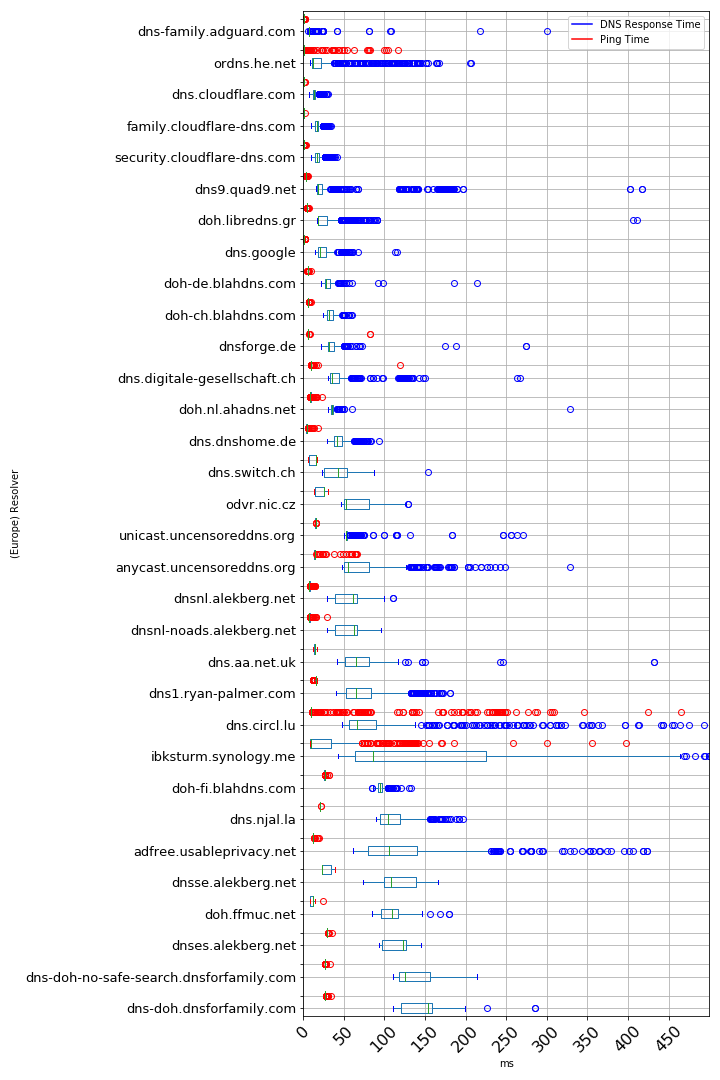
\includegraphics[height=2in]{figures/Frankfurt_Europe.png}}%
\caption{Resolvers measured from a vantage point in Frankfurt, Germany}
\end{figure}

\begin{figure}[t!]
\centering
\subfigure[North American resolvers measured from Ohio, USA]{%
\label{fig:Local_Ohio_NA}%
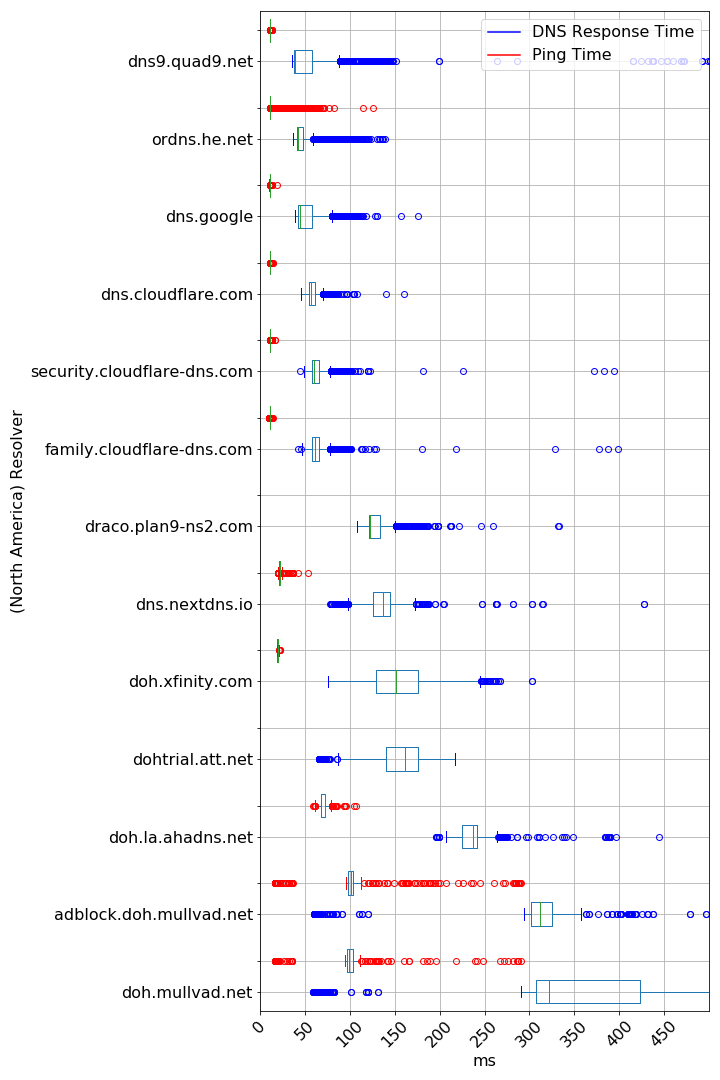
\includegraphics[height=2in]{figures/Ohio_North_America.png}}%
\hspace{8pt}%
\subfigure[Asian resolvers measured from Seoul, South Korea]{%
\label{fig:Local_Seoul_Asia}%
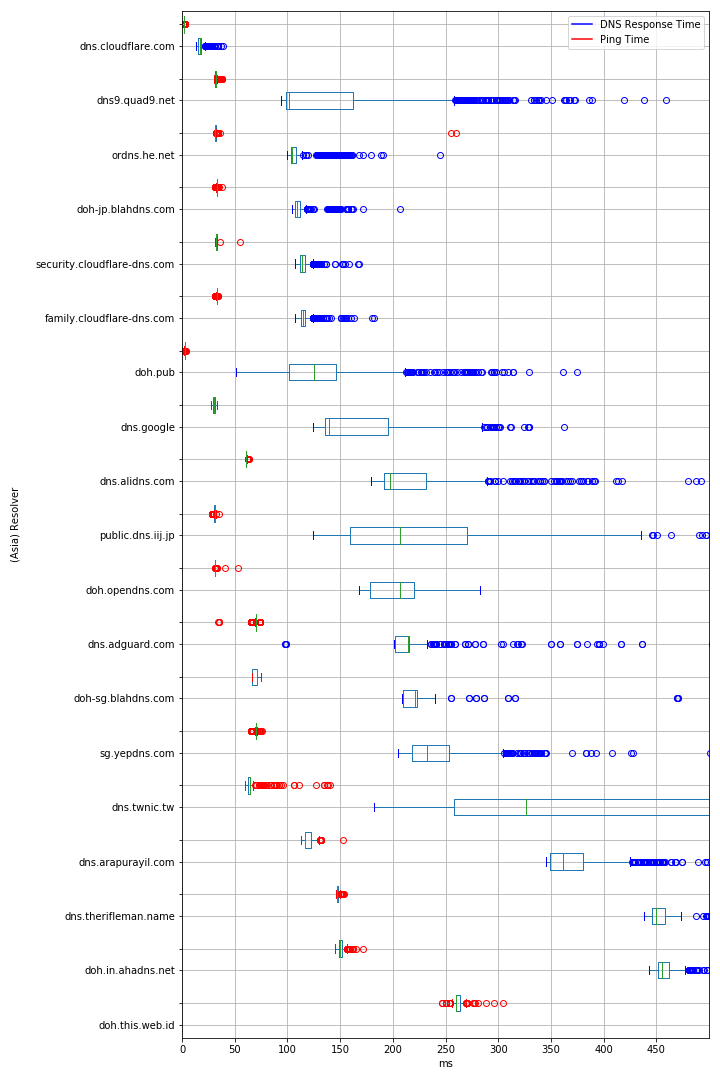
\includegraphics[height=2in]{figures/Seoul_Asia.png}}%
\hspace{8pt}%
\subfigure[European resolvers measured from Frankfurt, Germany]{%
\label{fig:Kocal_Frankfurt_Europe}%
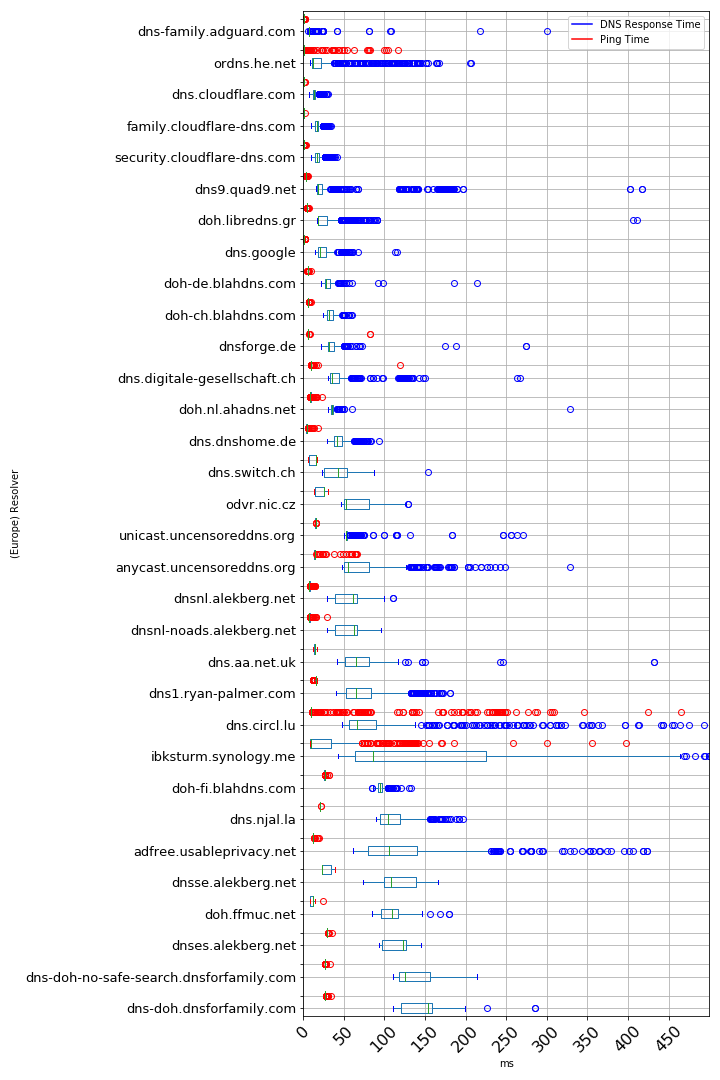
\includegraphics[height=2in]{figures/Frankfurt_Europe.png}}%
\caption{Local-to-local resolvers.}
\end{figure}

\begin{table}[t!]
\centering
\begin{tabular}{ll}
\hline
\textbf{Location} & \textbf{Resolver}                                                                               \\ \hline
North America     & ordns.he.net                                                                                    \\ \hline
Asia              & \begin{tabular}[c]{@{}l@{}}ordns.he.net\\ doh-jp.blahdns.com\end{tabular}                       \\ \hline
Europe            & \begin{tabular}[c]{@{}l@{}}ordns.he.net\\ dns-family.adguard.com\\ doh.libredns.gr\end{tabular} \\ \hline
\end{tabular}
\caption{Non-mainstream resolvers that outperformed mainstream resolvers.}
\label{tab:outperformed_resolvers}
\end{table}

\subsection{How Do Mainstream Resolvers Compare to Non-Mainstream Resolvers?}
We find that, in general, mainstream resolvers outperformed non-mainstream resolvers, with some notable exceptions.
Table~\ref{tab:outperformed_resolvers} compares median response times for major resolvers to non-mainstream resolvers that performed better.
Across all three vantage points, \texttt{dns.quad9.net}, \texttt{dns.google}, and \texttt{dns.cloudflare.com} were among the top five highest performing DoH resolvers.
However, \texttt{ordns.he.net}--a DoH resolver hosted by Hurricane Electric, a global Internet service provider (ISP)--managed to outperform \texttt{dns.google} and \texttt{dns.cloudflare.com} from all three vantage points.
From our vantage point in Frankfurt, we see that \texttt{dns-family.adguard.com} and \texttt{ordns.he.net} are the top two highest performing resolvers.
Finally, from our vantage point in Seoul, we see that \texttt{doh-jp.blahdns.com} outperforms \texttt{dns.google}.

However, most other non-mainstream DoH resolvers performed worse than mainstream resolvers, and they exhibited a wide distribution of median query response times.
For example, from our Ohio vantage point, we observe that outside of the top-five highest performing resolvers, median query response times ranged from \xxx{X} ms to \xxx{X} ms.
From our Seoul vantage point, median response times outside of the top five ranged from \xxx{X} ms to \xxx{X} ms.
We observe more consistent performance overall from our Frankfurt vantage point, but we still see median query response times outside the top five range from \xxx{X} ms to \xxx{X} ms.

\subsection{Does Network Distance Correlate to High Response Times from Non-Mainstream Resolvers?}
\begin{table}[t!]
\centering
\begin{tabular}{l|rr}
\toprule
    \textbf{Resolver} & \multicolumn{2}{c}{\textbf{Vantage Point}} \\
                  & \textrm{Seoul (ms)}         & \textrm{Frankfurt (ms)} \\
\midrule
dns.twnic.tw                                & 326.19 & 32,374.03                            \\
doh-jp.blahdns.com                          & 109.41                                           & 754.26                              \\
sg.yepdns.com                               & 232.69                                           & 540.19                              \\
public.dns.iij.jp                           & 206.37                                           & 506.05                              \\
doh-sg.blahdns                              & 221.41                                           & 498.76                              \\
\bottomrule
\end{tabular}
\caption{Median DNS response times for non-conventional resolvers located in Asia.}
\label{tab:UnconvAsia}
\end{table}

\begin{table}[t!]
\centering
\begin{tabular}{l|rr}
\toprule
\textbf{Resolver} & \multicolumn{2}{c}{\textbf{Vantage Point}} \\
                  & \textrm{Frankfurt (ms)}     & \textrm{Seoul (ms)} \\
\midrule
doh.ffmuc.net                               & 109.15 & 1,307.21                         \\
ibksturm.synology.me                        & 85.77 & 1,227.35                         \\
dns-doh-no-safe-search.dnsforfamily         & 125.74 & 1,150.63                         \\
dnsforge.de                                 & 32.17 & 1,029.92                         \\
dns-doh.dnsforfamily                        & 153.74 & 1,153.29                         \\
\bottomrule
\end{tabular}
\caption{Median DNS response times for non-conventional resolvers located in Europe.}
\label{tab:UnconvEur}
\end{table}

In general, we find that network distance correlates to higher median response times.
\Fref{tab:UnconvAsia} shows that non-conventional resolvers located in Asia perform better from the Seoul vantage point than the Frankfurt vantage point. 
Similarly, \Fref{tab:UnconvEur} demonstrates that the response times of European non-conventional resolvers measured from Frankfurt are much lower than the response times of those same resolvers measured from Seoul.

However, certain resolvers performed significantly worse than their network distance might imply.
For example, although the average latency we observed to \texttt{doh.in.ahadns.net} from our Seoul vantage point was \xxx{X} ms, the median query response time was \xxx{X} ms.
Similarly, from our Ohio vantage point, we observed an average latency to \texttt{doh.xfinity.com} of \texttt{X} ms, despite a median query response time of \xxx{X} ms.
We believe this could be attributed these non-mainstream resolvers having especially smaller caches than mainstream resolvers.
These resolvers may perform better in the future as more clients use them and populate their caches.
\AH{Review this previous hypothesis later}
We note that certain resolvers did not respond to our ICMP ping messages (\Fref{tab:unresponsive}).

\subsection{How Many Non-Mainstream Resolvers Are Responsive?}
\begin{table}[t!]
\centering
\begin{tabular}{lllll}
\hline
\textbf{Location} & \textbf{Resolver} & \textbf{Responsive?} & & \\
    & & \textbf{Ohio} & \textbf{Seoul} & \textbf{Frankfurt} \\
\midrule
North America     & \begin{tabular}[c]{@{}l@{}}dnscrypt.ca-1-doh\\ dnscrypt.ca-2-doh\\ doh-cleanbrowsing\\ doh.post-factum.tk\end{tabular} & \begin{tabular}[c]{@{}l@{}}\\ \\ \\ \end{tabular} & \begin{tabular}[c]{@{}l@{}}\\ \\ \\ \end{tabular} & \begin{tabular}[c]{@{}l@{}}\\ \\ \\ \end{tabular}    \\ \midrule
Asia              & \begin{tabular}[c]{@{}l@{}}doh.tiarap.org\\ jp.tiarap.org\\ doh.linuxsec\end{tabular} & \begin{tabular}[c]{@{}l@{}}\\ \\ \end{tabular}      & \begin{tabular}[c]{@{}l@{}}\\ \\ \end{tabular}      & \begin{tabular}[c]{@{}l@{}}\checkmark\ \checkmark\ \end{tabular}            \\ \midrule
Europe            & \begin{tabular}[c]{@{}l@{}}doh.bortzmeyer\\ doh.appliedprivacy\\ doh.chewbacca.meganerd.nl\\ doh.powerdns\end{tabular} & \begin{tabular}[c]{@{}l@{}}\\ \\ \\ \end{tabular} & \begin{tabular}[c]{@{}l@{}}\\ \\ \\ \end{tabular} & \begin{tabular}[c]{@{}l@{}}\\ \\ \\ \end{tabular} \\ \bottomrule
\end{tabular}
\caption{Resolvers that failed to respond from each vantage point.}
\label{tab:unresponsive}
\end{table}
\Fref{tab:unresponsive} list the DoH resolvers that we failed to receive a response from.
\Fref{tab:errors} also breaks down the most common errors we received from attempting to communicate with unresponsive resolvers.
We find that most resolvers we measured were responsive, albeit some reported relatively high median query response times.
For the resolvers that we did not receive responses from, the most common errors related to a failure to establish a TCP connection or a TLS session.
\AH{Review this previous sentence later with the full data}
In other words, when we didn't receive a response, it wasn't necessarily because the response itself was dropped on-path or our software reported a timeout, but rather that the server was likely no longer operational in the first place.
